```tex
\documentclass{article}
\usepackage{amsmath, amssymb, graphicx, tikz, pgfplots, booktabs, xcolor}
\pgfplotsset{compat=1.18}

\newenvironment{lesson-meta}{}{}        % lesson code, title, objective, EQ, vocab
\newenvironment{item-analysis}{}{}      % Savvas's Example × DOK table
\newenvironment{model-discuss}{}{}      % Launch opener
\newenvironment{concept-box}{}{}        % in-lesson concept reference
\newenvironment{concept-summary}{}{}    % end-of-lesson summary
\newenvironment{example}[1]{}{}         % #1 = example number
\newenvironment{tryit}[1]{}{}           % #1 = tryit number
\newenvironment{practice}[2]{}{}        % #1 = practice number, #2 = DOK
\newenvironment{te-addendum}[2]{}{}     % #1 = anchor example, #2 = type
\newcommand{\answer}[1]{}               % answer key, inside any env
\newcommand{\placeholder}[2]{}          % #1 = type, #2 = description
\newcommand{\uncertain}[2]{#1}          % #1 = best guess, #2 = alternatives
\newcommand{\te}[1]{}                   % teacher-only inline annotation

\begin{document}

\begin{lesson-meta}
Lesson Code: 5-1

Title: nth Roots, Radicals, and Rational Exponents

I CAN: relate roots and rational exponents and use them to simplify expressions and solve equations.

Essential Question: How are exponents and radicals used to represent roots of real numbers?

Essential Understanding: A rational exponent has an equivalent radical expression and any radical expression may be written with a rational exponent. This foundation is necessary to simplify expressions and solve equations.

Lesson Vocabulary: nth root

Topic Vocabulary: complex conjugate, exponent, index, radical symbol, radicand
\end{lesson-meta}

\begin{item-analysis}
\begin{tabular}{ccc}
\toprule
Example & Items & DOK \\
\midrule
1 & 25--28 & 1 \\
1 & 22 & 2 \\
2 & 29--32, 48 & 1 \\
2 & 20, 21, 24, 47 & 2 \\
3 & 33--34 & 1 \\
4 & 35--38, 49 & 1 \\
4 & 18 & 2 \\
5 & 39--42 & 1 \\
6 & 19, 23, 43--46 & 2 \\
6 & 50 & 3 \\
\bottomrule
\end{tabular}
\end{item-analysis}

\begin{model-discuss}
EXPLORE \& REASON

The graph shows \(y=x^2\).

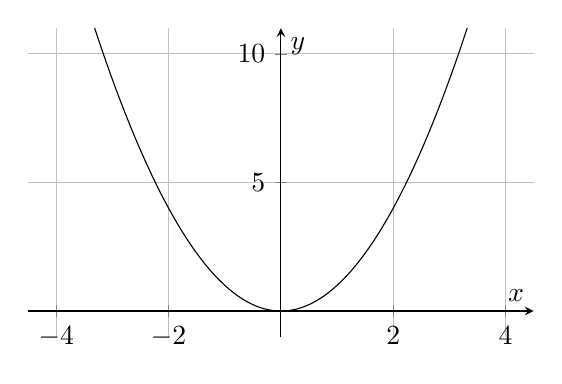
\begin{tikzpicture}
\begin{axis}[
    width=8cm,
    height=5.5cm,
    axis lines=middle,
    xlabel={$x$},
    ylabel={$y$},
    xmin=-4.5, xmax=4.5,
    ymin=-1, ymax=11,
    xtick={-4,-2,0,2,4},
    ytick={0,5,10},
    grid=both,
]
\addplot[domain=-4:4, samples=100] {x^2};
\end{axis}
\end{tikzpicture}

A. Find all possible values of \(x\) or \(y\) so that the point is on the graph.

\[
\begin{array}{ll}
\text{(a) }(2,\_\_\_) & \text{(b) }(3,\_\_\_)\\
\text{(c) }(-3,\_\_\_) & \text{(d) }(5,\_\_\_)\\
\text{(e) }(\_\_\_,4) & \text{(f) }(\_\_\_,-16)\\
\text{(g) }(\_\_\_,7) & \text{(h) }(\_\_\_,5)
\end{array}
\]

\answer{A. a. 4; b. 9; c. 9; d. 25; e. \(-2,2\); f. no possible value; g. \(-\sqrt{7},\sqrt{7}\); h. \(-\sqrt{5},\sqrt{5}\).}

B. Communicate Precisely Write a precise set of instructions that show how to find an approximate value of \(\sqrt{13}\) using the graph.

\answer{Draw the line \(y=13\) on the graph. Draw a vertical line from where the horizontal line intersects the graph down to the positive \(x\)-axis, and read the corresponding value.}

C. Draw a graph of \(y=x^3\). Use the graph to approximate each value.

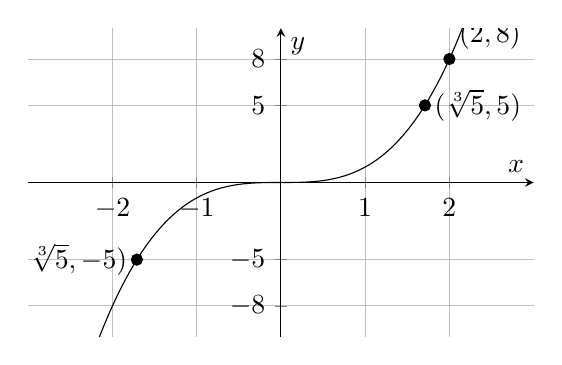
\begin{tikzpicture}
\begin{axis}[
    width=8cm,
    height=5.5cm,
    axis lines=middle,
    xlabel={$x$},
    ylabel={$y$},
    xmin=-3, xmax=3,
    ymin=-10, ymax=10,
    xtick={-2,-1,0,1,2},
    ytick={-8,-5,0,5,8},
    grid=both,
]
\addplot[domain=-2.2:2.2, samples=100] {x^3};
\addplot[only marks] coordinates {(1.71,5) (-1.71,-5) (2,8)};
\node at (axis cs:1.71,5) [anchor=west] {$(\sqrt[3]{5},5)$};
\node at (axis cs:-1.71,-5) [anchor=east] {$(-\sqrt[3]{5},-5)$};
\node at (axis cs:2,8) [anchor=south west] {$(2,8)$};
\end{axis}
\end{tikzpicture}

\[
\begin{array}{lll}
\text{(a) }\sqrt[3]{5} & \text{(b) }\sqrt[3]{-5} & \text{(c) }\sqrt[3]{8}\\
\text{(d) A solution to }x^3=5 & \text{(e) A solution to }x^3=-5 & \text{(f) A solution to }x^3=8
\end{array}
\]

\answer{C. a. \(\approx 1.7\); b. \(\approx -1.7\); c. \(2\); d. \(\approx 1.7\); e. \(\approx -1.7\); f. \(2\).}
\end{model-discuss}

\begin{te-addendum}{ExploreAndReason}{LearnTogether}
Before, Implement Tasks that Promote Reasoning and Problem Solving

Q: What do you notice about the graph of \(y=x^2\)?

\answer{The graph is a parabola. All values of \(y\) are greater than or equal to zero.}
\end{te-addendum}

\begin{te-addendum}{ExploreAndReason}{LearnTogether}
During, Support Productive Struggle in Learning Mathematics

Q: What is true about the possible missing \(x\)-values compared to the possible missing \(y\)-values?

\answer{For every ordered pair that is missing an \(x\)-value, there are 2 possible values for \(x\). For every ordered pair that is missing a \(y\)-value, there is only 1 possible value for \(y\).}
\end{te-addendum}

\begin{te-addendum}{ExploreAndReason}{RtIExtend}
For Early Finishers

Q: Draw a graph of \(y=x^4\) and \(y=x^5\). Use the graphs to find approximate values as in Part C. How do the numbers of \(x\)- and \(y\)-values compare to the numbers of \(x\)- and \(y\)-values of the graphs of \(y=x^2\) and \(y=x^3\)?

\answer{Each \(y\)-value for \(y=x^4\) has 2 possible \(x\)-values, like \(y=x^2\). Each \(y\)-value for \(y=x^5\) has 1 possible \(x\)-value, like \(y=x^3\).}
\end{te-addendum}

\begin{te-addendum}{ExploreAndReason}{LearnTogether}
After, Facilitate Meaningful Mathematical Discourse

Q: Can the instructions you created in Part B be used to approximate the cube root of a number?

\answer{Yes; the instructions also work for finding cube roots. Use the graph to find a point with a \(y\)-value that is placed under the radical sign. Then find the cube root to find the corresponding \(x\)-value of that point.}

Q: What do you notice about the answers in Part C?

\answer{The value for \(\sqrt[3]{5}\) is the same as the solution to \(x^3=5\), the value for \(\sqrt[3]{-5}\) is the same as the solution to \(x^3=-5\), and the value for \(\sqrt[3]{8}\) is the same as the solution to \(x^3=8\).}
\end{te-addendum}

\begin{te-addendum}{ExploreAndReason}{HabitsOfMind}
Look for Relationships How is \(\sqrt{5}\) related to 5? How is \(\sqrt[3]{5}\) related to 5? How do you think \(\sqrt[4]{5}\) is related to 5?

\answer{\((\sqrt{5})^2=5\); \((\sqrt[3]{5})^3=5\); \((\sqrt[4]{5})^4=5\).}
\end{te-addendum}

\begin{example}{1}
Find All Real nth Roots

A. What are all the real cube roots of 125?

An \(n\)th root of a number \(c\) is \(x\), such that \(x^n=c\). An \(n\)th root can be represented using a radical symbol by \(x=\sqrt[n]{c}\).

Since \(125=5^3\), \(\sqrt[3]{125}=5\) is a real cube root.

To determine if there are other real cube roots of 125, consider the function \(f(x)=x^3-125\). The zeroes of \(f\) are the cube roots of 125.

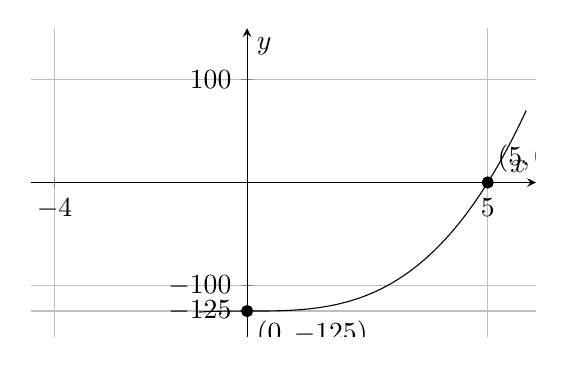
\begin{tikzpicture}
\begin{axis}[
    width=8cm,
    height=5.5cm,
    axis lines=middle,
    xlabel={$x$},
    ylabel={$y$},
    xmin=-4.5, xmax=6,
    ymin=-150, ymax=150,
    xtick={-4,0,5},
    ytick={-125,-100,0,100},
    grid=both,
]
\addplot[domain=-1:5.8, samples=100] {x^3-125};
\addplot[only marks] coordinates {(5,0) (0,-125)};
\node at (axis cs:5,0) [anchor=south west] {$(5,0)$};
\node at (axis cs:0,-125) [anchor=north west] {$(0,-125)$};
\end{axis}
\end{tikzpicture}

The graph of \(f\) has only one \(x\)-intercept. Therefore, 5 is the only real cube root of 125.

B. What are all the real fourth roots of 16?

Since \(16=2^4\), one fourth root is the principal root, \(\sqrt[4]{16}=2\).

To determine all the real fourth roots of 16, solve \(x^4=16\).

\[
\begin{aligned}
x^4&=16\\
x^4-16&=0\\
(x^2-4)(x^2+4)&=0\\
(x-2)(x+2)(x^2+4)&=0
\end{aligned}
\]

The zeros of the first two factors are 2 and \(-2\). The zeros of the quadratic factor \(x^2+4\) are imaginary. Therefore, the real fourth roots of 16 are 2 and \(-2\).

\answer{A. 5 is the only real cube root of 125. B. The real fourth roots of 16 are 2 and \(-2\).}
\end{example}

\begin{tryit}{1}
Find the specified roots of each number.

a. real fourth roots of 81

b. real cube roots of 64

\answer{a. \(\pm 3\); b. 4}
\end{tryit}

\begin{te-addendum}{1}{PurposefulQuestions}
Q: When finding the \(n\)th root of a number, what do you notice about the real and complex solutions?

\answer{The sum of the number of real and complex solutions is \(n\).}

Q: How are the real roots of an even power related?

\answer{The real roots of an even power are opposites.}
\end{te-addendum}

\begin{te-addendum}{1}{ElicitEvidence}
Q: What do you know about the roots of a number before you solve the problem?

\answer{If the degree is odd, there will be an odd number of real roots. If the degree is even, there will be an even number of real roots.}
\end{te-addendum}

\begin{te-addendum}{1}{CommonError}
Try It! 1a When finding the real fourth roots of 81, students may give the root as 3. Have students find the square roots of 81, reminding them that there are two real roots. Then ask students how this is related to finding the real fourth roots of 81.
\end{te-addendum}

\begin{te-addendum}{1}{LearnTogether}
Additional Example 1

Find the real fourth roots of \(-256\).

\[
\begin{aligned}
x^4&=-256\\
x^4+256&=0
\end{aligned}
\]

\(x^4+256=0\) does not have real solutions.

Therefore, there are no real fourth roots of \(-256\).

\answer{There are no real fourth roots of \(-256\).}
\end{te-addendum}

\begin{te-addendum}{1}{PurposefulQuestions}
Example 1 Help students find the real cube and fourth roots of a negative number.

Q: Can you find the real cube and fourth roots of a negative number?

\answer{You can find the cube root of a negative number, but there is no real number that when raised to the fourth power results in a negative number.}
\end{te-addendum}

\begin{example}{2}
Understand Rational Exponents

A. What is the meaning of the exponent in the expression \(16^{\frac14}\)?

Extend the properties of integer exponents to rational exponents.

\[
\begin{aligned}
16^{\frac14}&=(2^4)^{\frac14} && \text{Use the Power of a Power Property.}\\
&=2^1\\
&=\sqrt[4]{16} && \text{Since }2=\sqrt[4]{16},\ 16=2^4.
\end{aligned}
\]

Therefore, \(16^{\frac14}\) is another way to represent \(\sqrt[4]{16}\), or 2.

In general, for positive integer \(n\), \(x^{\frac1n}\) can be expressed as the radical \(\sqrt[n]{x}\).

\[
x^{\frac1n}=\sqrt[n]{x}
\]

Both the exponent \(\frac1n\) and the radical symbol \(\sqrt[n]{}\) indicate the principal \(n\)th root.

B. Write \(27^{\frac23}\) as a radical.

\[
\begin{aligned}
27^{\frac23}&=\left(27^{\frac13}\right)^2 && \text{Use the Power of a Power Property.}\\
&=\left(\sqrt[3]{27}\right)^2\\
&=3^2\\
&=9
\end{aligned}
\]

This means that you can rewrite \(27^{\frac23}\) as \(\left(\sqrt[3]{27}\right)^2\). Since 27 is a perfect cube, you can evaluate the radical expression mentally by taking the cube root first and then squaring.

\[
27^{\frac23}=\left(\sqrt[3]{27}\right)^2=3^2=9
\]

\answer{A. \(16^{\frac14}\) means the fourth root of 16; \(16^{\frac14}=2\). B. \(27^{\frac23}=\left(\sqrt[3]{27}\right)^2=9\).}
\end{example}

\begin{tryit}{2}
Explain what each fractional exponent means, then evaluate.

a. \(25^{\frac12}\)

b. \(32^{\frac25}\)

\answer{a. square root of 25; 5. b. fifth root of 32 squared; 4.}
\end{tryit}

\begin{te-addendum}{2}{PurposefulQuestions}
Q: Does the order in which you raise a number to a power and find the \(n\)th root matter?

\answer{No; you can raise a number to a power and then take the \(n\)th root, or you can take the \(n\)th root and then raise that number to a power.}

Q: Assuming that \(x\) is a real number, what do you know about the value of \(n\) if \(x\) is negative?

\answer{If \(x\) is negative, the value of \(n\) is an odd number, because you cannot find real \(n\)th roots of a negative number if \(n\) is even.}

Q: Could a rational exponent have a 1 in the denominator? What does that represent?

\answer{A rational exponent can have a 1 in the denominator. A rational exponent with a 1 in the denominator would be the same as an exponent with an integer value.}
\end{te-addendum}

\begin{te-addendum}{2}{ElicitEvidence}
Q: What do the numerator and denominator of a rational exponent represent?

\answer{The numerator is the power that the number is raised to. The denominator is the root of the number you are finding.}
\end{te-addendum}

\begin{te-addendum}{2}{HabitsOfMind}
Generalize If a base raised to a fractional exponent is imaginary, what is true about the values of the numbers involved?

\answer{The base is negative, and the denominator of the fractional exponent must be even.}
\end{te-addendum}

\begin{te-addendum}{2}{ELLAddendum}
READING BEGINNING Write the following sentences on the board and help students to read them. Laughter is an expression of emotion. He sat there with an expression of sadness on his face. Although her voice was quiet, her expression reflected strength.

Q: Using context clues, what does the word expression mean in the sentences you read?

\answer{A way of communicating, or representing, emotions without speaking.}

Q: Have students read the first sentence of both parts (a) and (b). What does the word expression mean in the example?

\answer{Numbers and symbols that show a value.}

LISTENING DEVELOPING Students may think of power as the possession of control over others, as illustrated in the following sentence. Read this sentence aloud: The highest power in our country is held by the president. Then read the example aloud as students listen.

Q: Does power mean the same thing in the example as it does in the sentence you heard?

\answer{No.}

Q: What other word did you hear in the example that means the same thing as power?

\answer{Exponent.}

Q: Listen to the first sentence again. What is the exponent? What is the power?

\answer{\(\frac14\); \(\frac14\). Exponent and power are synonyms.}

WRITING EXPANDING Write the following sentences on the board: Do you own any property? One property of gold is that it is a soft metal.

Q: What does the word property mean in the first sentence?

\answer{A piece of land that a person owns.}

Q: What does the word property mean in the second sentence?

\answer{A characteristic that describes something.}

Q: How does the second definition help you understand how the term property is used in math?

\answer{Math properties describe the characteristics of numbers and their relationships.}
\end{te-addendum}

\begin{concept-box}
Interpreting Rational Exponents

In general, if the \(n\)th root of \(c\) is a real number,
\[
\sqrt[n]{c}=c^{\frac1n}.
\]

Furthermore, if \(m\) is an integer, then
\[
c^{\frac mn}=\left(c^{\frac1n}\right)^m=\left(\sqrt[n]{c}\right)^m
\quad\text{and}\quad
\sqrt[n]{c^m}=\left(c^m\right)^{\frac1n}=c^{\frac mn}.
\]
\end{concept-box}

\begin{example}{3}
Evaluate Expressions With Rational Exponents

A. Evaluate the expressions \(32^{\frac35}\), \(27^{-\frac23}\), and \(50^{\frac34}\).

\[
\begin{aligned}
32^{\frac35}&=\left(32^{\frac15}\right)^3\\
&=2^3\\
&=8
\end{aligned}
\qquad
\begin{aligned}
27^{-\frac23}&=\left(27^{\frac13}\right)^{-2}\\
&=(3)^{-2}\\
&=\frac19
\end{aligned}
\]

Since 50 does not have a perfect 4th root, use a calculator to approximate:
\[
50^{\frac34}\approx 18.80.
\]

B. The Fujita scale rating, \(F\), of a tornado is represented by
\[
F=\sqrt[3]{\left(\frac{W}{14.1}\right)^2}-2,
\]
where \(W\) is the estimated wind speed of the tornado in miles per hour. What is the Fujita scale rating for this tornado?

\placeholder{photo}{Tornado over a road with a label pointing to the funnel cloud: "Wind speed estimated at 100 mph"}

\[
\begin{aligned}
F&=\sqrt[3]{\left(\frac{100}{14.1}\right)^2}-2\\
&=\left(\frac{100}{14.1}\right)^{\frac23}-2\\
&\approx (7.09)^{\frac23}-2\\
&\approx 3.69-2\\
&\approx 1.69
\end{aligned}
\]

A tornado with estimated wind speeds of 100 mph is classified as F1 according to the Fujita scale.

\answer{A. \(8\), \(\frac19\), and approximately \(18.80\). B. F1.}
\end{example}

\begin{tryit}{3}
What is the value of each expression? Round to the nearest hundredth if necessary.

a. \(-\left(16^{\frac34}\right)\)

b. \(\sqrt[5]{3.5^4}\)

\answer{a. \(-8\); b. \(2.72\).}
\end{tryit}

\begin{te-addendum}{3}{PurposefulQuestions}
Q: Why might it be easier to calculate the \(n\)th root before raising to a power?

\answer{When you calculate the \(n\)th root first, the number that you raise to a power is smaller, so the calculation is easier.}

Q: What is another method you could use to evaluate an expression that has a negative rational exponent?

\answer{You can rewrite the base of the exponent as its reciprocal before or after calculating the root and power.}

Q: How is the Fujita scale classification related to the value of \(F\) you calculated?

\answer{The number in the Fujita scale classification is equal to the integer part of the value calculated.}

Q: Why is a calculator a useful tool when approximating a cube root?

\answer{If the cube root is not a perfect cube, it is difficult to accurately approximate the value.}
\end{te-addendum}

\begin{te-addendum}{3}{ElicitEvidence}
Q: In Part A, does it matter in what order you apply the negative?

\answer{Because the power is within parentheses, you must evaluate the power before applying the negative.}
\end{te-addendum}

\begin{te-addendum}{3}{RtIExtend}
Extend Student Thinking

USE WITH EXAMPLE 3 Have students explore finding the value of more complicated expressions that contain rational exponents, expanding their use of rational exponents across the different properties of exponents.

What is the value of each expression?

1. \(27^{\frac43}+8-8^{\frac23}\)

\answer{85}

2. \(4^{\frac52}+5-16^{\frac32}\)

\answer{\(-27\)}

3. \(3(8)^{-\frac13}+5+4^{-\frac12}\)

\answer{7}

4. \(\left(\frac{8}{27}\right)^{-\frac13}-6-\left(\frac{81}{16}\right)^{\frac14}\)

\answer{\(-6\)}

5. \(\left(64^{\frac13}\right)^{\frac52}\)

\answer{32}
\end{te-addendum}

\begin{example}{4}
Simplify nth Roots

Simplify each expression. Assume all variables are positive.

A. \(\sqrt[5]{32m^{15}}\)

\[
\begin{aligned}
\sqrt[5]{2^5m^{15}}&=\sqrt[5]{(2m^3)^5}\\
&=2m^3
\end{aligned}
\]

So, \(\sqrt[5]{32m^{15}}=2m^3\).

B. \(\sqrt[4]{x^{20}y^8}\)

\[
\begin{aligned}
\sqrt[4]{x^{20}y^8}&=(x^{20}y^8)^{\frac14}\\
&=x^{\frac{20}{4}}y^{\frac84}\\
&=x^5y^2
\end{aligned}
\]

So, \(\sqrt[4]{x^{20}y^8}=x^5y^2\).

\answer{A. \(2m^3\); B. \(x^5y^2\).}
\end{example}

\begin{tryit}{4}
Simplify each expression.

a. \(\sqrt[3]{-8a^3b^9}\)

b. \(\sqrt[4]{256x^{12}y^{24}}\)

\answer{a. \(-2ab^3\); b. \(4x^3y^6\).}
\end{tryit}

\begin{te-addendum}{4}{PurposefulQuestions}
PART A

Q: What is another approach you can use to simplify the expression?

\answer{You can write the 5th root as the rational exponent. Then multiply the exponent of each factor by the rational exponent and simplify.}

PART B

Q: Why is it necessary to assume all variables represent positive numbers?

\answer{Because the given expression uses the radical symbol, which represents the principal (positive) root, it can only be equivalent to an expression with a nonnegative value. The exponent of \(x^5\) is odd, so the value of \(x^5\) could be negative. In this case, the expression \(x^5y^2\) would not be equivalent to the given expression because it would be negative. Using variables to represent only positive numbers ensures that the resulting expression is nonnegative and thus equivalent to the given expression.}
\end{te-addendum}

\begin{te-addendum}{4}{ElicitEvidence}
Q: Why is it important to write the radicand as an expression to a power before evaluating?

\answer{Rewriting as an expression to a power makes it simpler to find the \(n\)th root.}
\end{te-addendum}

\begin{te-addendum}{4}{HabitsOfMind}
Make Sense and Persevere What is an example of a variable expression that has both a cube root and a fourth root, which can be simplified to an expression without a radical?

\answer{Answers will vary. Sample: \(x^{12}\).}
\end{te-addendum}

\begin{te-addendum}{4}{RtISupport}
Support Struggling Students

USE WITH EXAMPLE 4 Students may have difficulty simplifying expressions with \(n\)th roots. Have students practice simplifying expressions with square roots.

Simplify each expression. Assume all variables are positive.

1. \(\sqrt{4a^4}\)

\answer{\(2a^2\)}

2. \(\sqrt{49y^6z^2}\)

\answer{\(7y^3z\)}

3. \(\sqrt{121m^8n^4}\)

\answer{\(11m^4n^2\)}
\end{te-addendum}

\begin{example}{5}
Use nth Roots to Solve Equations

Solve the equation \(2x^5=64\).

A.
\[
\begin{aligned}
2x^5&=64\\
x^5&=32\\
(x^5)^{\frac15}&=32^{\frac15}\\
x&=2
\end{aligned}
\]

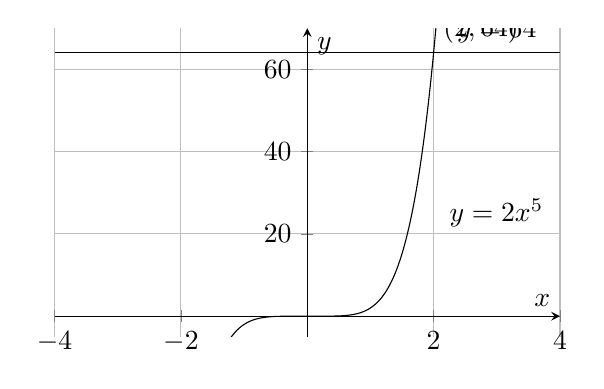
\begin{tikzpicture}
\begin{axis}[
    width=8cm,
    height=5.5cm,
    axis lines=middle,
    xlabel={$x$},
    ylabel={$y$},
    xmin=-4, xmax=4,
    ymin=-5, ymax=70,
    xtick={-4,-2,0,2,4},
    ytick={0,20,40,60},
    grid=both,
]
\addplot[domain=-2:2.2, samples=100] {2*x^5};
\addplot[domain=-4:4, samples=2] {64};
\node at (axis cs:2,64) [anchor=south west] {$(2,64)$};
\node at (axis cs:3,64) [anchor=south] {$y=64$};
\node at (axis cs:2.1,25) [anchor=west] {$y=2x^5$};
\end{axis}
\end{tikzpicture}

The graph shows one point of intersection, so there is only one real solution.

The solution to the equation is \(x=2\).

B.
\[
\begin{aligned}
3x^4&=1875\\
x^4&=625\\
(x^4)^{\frac14}&=\pm(625)^{\frac14}\\
x&=\pm5
\end{aligned}
\]

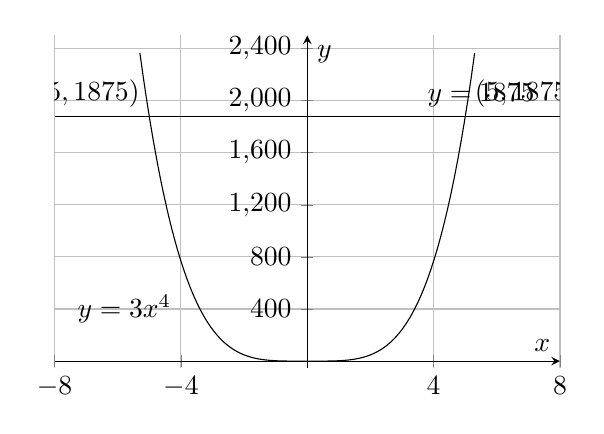
\begin{tikzpicture}
\begin{axis}[
    width=8cm,
    height=5.8cm,
    axis lines=middle,
    xlabel={$x$},
    ylabel={$y$},
    xmin=-8, xmax=8,
    ymin=-50, ymax=2500,
    xtick={-8,-4,0,4,8},
    ytick={0,400,800,1200,1600,2000,2400},
    grid=both,
]
\addplot[domain=-5.3:5.3, samples=100] {3*x^4};
\addplot[domain=-8:8, samples=2] {1875};
\node at (axis cs:-5,1875) [anchor=south east] {$(-5,1875)$};
\node at (axis cs:5,1875) [anchor=south west] {$(5,1875)$};
\node at (axis cs:5.5,1875) [anchor=south] {$y=1875$};
\node at (axis cs:-4,400) [anchor=east] {$y=3x^4$};
\end{axis}
\end{tikzpicture}

The graphs show 2 points of intersection, so there are no other real solutions.

The solutions are \(x=\pm5\).

\answer{A. \(x=2\). B. \(x=\pm5\).}
\end{example}

\begin{tryit}{5}
a. Solve the equation \(5x^3=320\).

b. Solve the equation \(2p^4=162\).

\answer{a. \(x=4\); b. \(p=\pm3\).}
\end{tryit}

\begin{te-addendum}{5}{PurposefulQuestions}
Q: What property are you using when you rewrite \((x^5)^{\frac15}\) as \(x\)?

\answer{The Power of a Power Property.}
\end{te-addendum}

\begin{te-addendum}{5}{ElicitEvidence}
Q: What do you notice about these equations that makes them easier to solve?

\answer{The coefficient of the variable divides the value on the other side of the equation evenly. In part (a), this quotient is a perfect cube. In part (b), this quotient is a perfect fourth power.}
\end{te-addendum}

\begin{concept-box}
Solving an Equation in the Form \(x^n=c\)

To solve an equation in the form \(x^n=c\), find the \(n\)th root of both sides by raising each expression to the \(\frac1n\) power.

\[
(x^n)^{\frac1n}=(c)^{\frac1n}
\]
\end{concept-box}

\begin{example}{6}
Use nth Roots to Solve Problems

A garden water fountain is made of two cubes. The larger container has an edge length 2 cm longer than the edge length of a second cube. When the larger cube empties into the smaller cube, how much water will spill over the edge of the smaller cube into the base?

\placeholder{illustration}{Garden water fountain made of two cubes. Water pours from a larger upper cube into a smaller lower cube. Label: "The volume of the larger cube is 729 cm^3."}

\[
\begin{aligned}
(x+2)^3&=729\\
\left[(x+2)^3\right]^{\frac13}&=(729)^{\frac13}\\
x+2&=9\\
x&=7
\end{aligned}
\]

The volume of the smaller cube is \(7^3\), or \(343\text{ cm}^3\).

The volume of the larger cube is \(729\text{ cm}^3\).

The amount of water that spills is \(729-343=386\).

When the larger cube empties into the smaller cube, \(386\text{ cm}^3\) of water will spill out into the base of the fountain.

\answer{\(386\text{ cm}^3\)}
\end{example}

\begin{tryit}{6}
One cube has an edge length 3 cm shorter than the edge length of a second cube. The volume of the smaller cube is \(200\text{ cm}^3\). What is the volume of the larger cube?

\answer{\(\approx 692.69\text{ cm}^3\)}
\end{tryit}

\begin{te-addendum}{6}{PurposefulQuestions}
Use and Connect Mathematical Representations

Q: What does volume mean in the context of this problem?

\answer{The volume is the amount of water that a cube can hold.}

Q: What do you notice about the image that is important to understanding and solving this problem?

\answer{The top cube is larger than the smaller cube. To find the difference of the volumes of the cubes, you have to subtract the volume of the smaller cube from the volume of the larger cube.}
\end{te-addendum}

\begin{te-addendum}{6}{ElicitEvidence}
Q: Is the edge length of the smaller cube an integer? How can you tell without solving?

\answer{No; you can tell because the value of the volume, \(200\text{ cm}^3\), is not a perfect cube.}
\end{te-addendum}

\begin{te-addendum}{6}{HabitsOfMind}
Communicate Precisely What are the steps necessary to solve the equation \(ax^n=b\)?

\answer{Divide both sides of the equation by \(a\) to isolate the \(x\)-term. Then take the \(n\)th root of both sides so you have \(x=\sqrt[n]{\frac ba}\).}
\end{te-addendum}

\begin{te-addendum}{6}{LearnTogether}
Additional Example 6

A clerk is wrapping two cube-shaped packages and wants to know the smallest amount of wrapping paper that can wrap each package. The edge length of the larger package is 3 in. greater than the edge length of the smaller package. The surface area of the larger package is \(384\text{ in.}^2\). What is the surface area of the smaller package?

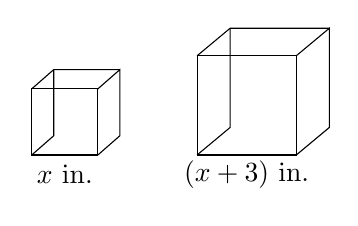
\begin{tikzpicture}[scale=0.7]
\draw (0,0) rectangle (1.2,1.2);
\draw (1.2,0) -- (1.6,0.35) -- (1.6,1.55) -- (1.2,1.2);
\draw (0,1.2) -- (0.4,1.55) -- (1.6,1.55);
\draw (0.4,1.55) -- (0.4,0.35) -- (0,0);
\node at (0.6,-0.35) {\(x\) in.};

\begin{scope}[xshift=3cm]
\draw (0,0) rectangle (1.8,1.8);
\draw (1.8,0) -- (2.4,0.5) -- (2.4,2.3) -- (1.8,1.8);
\draw (0,1.8) -- (0.6,2.3) -- (2.4,2.3);
\draw (0.6,2.3) -- (0.6,0.5) -- (0,0);
\node at (0.9,-0.35) {\((x+3)\) in.};
\end{scope}
\end{tikzpicture}

\[
\begin{aligned}
384&=6(x+3)^2\\
64&=(x+3)^2\\
8&=x+3\\
5&=x
\end{aligned}
\]

The side length of the smaller cube is 5 in.

\[
6(5)^2=6(25)=150
\]

So, the surface area of the smaller cube is \(150\text{ in.}^2\).

\answer{\(150\text{ in.}^2\)}
\end{te-addendum}

\begin{te-addendum}{6}{PurposefulQuestions}
Example 6 Help students use \(n\)th roots to find the edge length of a cube, given the surface area.

Q: What is the value of \(n\) in the \(n\)th root in this example?

\answer{2}

Q: Why is the expression \(6s^2\) used to find the surface area of a cube?

\answer{The area of a face of a cube is equal to \(s^2\) and there are 6 faces on a cube.}
\end{te-addendum}

\begin{concept-summary}
CONCEPT SUMMARY nth Roots, Radicals, and Rational Exponents

Relating Radical and Exponential Forms

\begin{tabular}{lll}
\toprule
 & Radical Form & Exponential Form \\
\midrule
Numbers & \(\sqrt[5]{32^4}=(32^4)^{\frac15}=32^{\frac45}\) & \(729^{\frac56}=(729^{\frac16})^5=(\sqrt[6]{729})^5\) \\
Algebra & \(\sqrt[n]{c^m}=(c^m)^{\frac1n}=c^{\frac mn}\) & \(c^{\frac mn}=(c^{\frac1n})^m=\sqrt[n]{c^m}\) \\
\bottomrule
\end{tabular}

The index of a radical is equivalent to the denominator of a fractional exponent. The exponent of the radicand is equivalent to the numerator of a fractional exponent.

Solving an Equation in the Form \(x^n=c\)

To solve an equation in the form \(x^n=c\), find the \(n\)th root of both sides of the equation by raising each expression to the \(\frac1n\) power.

\[
\begin{aligned}
x^3&=1,728\\
(x^3)^{\frac13}&=(1,728)^{\frac13}\\
x&=12
\end{aligned}
\]

\[
\begin{aligned}
x^n&=c\\
(x^n)^{\frac1n}&=(c)^{\frac1n}\\
x&=c^{\frac1n}
\end{aligned}
\]

Do You UNDERSTAND?

1. ESSENTIAL QUESTION How are exponents and radicals used to represent roots of real numbers?

\answer{A radical can be rewritten as a fractional exponent, where the index is the denominator of the exponent. Both a radical with index \(n\) and a fractional exponent \(\frac1n\) represent the \(n\)th root of a real number.}

2. Error Analysis Kaitlyn said \(\sqrt[3]{10}=10^3\). Explain Kaitlyn's error.

\answer{Kaitlyn made the exponent equal to the index. The index should be the denominator of the exponent, so the exponent should be \(\frac13\).}

3. Vocabulary In the radical expression \(\sqrt[5]{125}\), what is the index? What is the radicand?

\answer{The index is 5 and the radicand is 125.}

4. Use Structure Why is \(75^{\frac35}\) equal to \(\left(75^{\frac15}\right)^3\)?

\answer{\(\left(75^{\frac15}\right)^3\) can be simplified using the Power of a Power Property. Multiplying the exponents gives \(75^{\frac35}\).}

5. Construct Arguments Amani said that \((x^8)^{\frac14}=\frac{x^8}{x^4}=x^4\). Is Amani correct? Explain.

\answer{No; Amani did not apply the Power of a Power Property correctly; \((x^8)^{\frac14}=x^{8\cdot \frac14}=x^2\).}

6. Make Sense and Persevere Is it possible for a rational exponent to be an improper fraction? Explain how \(27^{\frac43}\) is evaluated or why it cannot be evaluated.

\answer{Yes, a rational exponent may be an improper fraction; \(27^{\frac43}\) is evaluated by finding the cube root of 27, which is 3, and raising it to the fourth power, which is 81.}

Do You KNOW HOW?

Write each expression in radical form.

7. \(a^{\frac15}\)

\answer{\(\sqrt[5]{a}\)}

8. \(7^{\frac23}\)

\answer{\(\sqrt[3]{7^2}\)}

Write each expression in exponential form.

9. \(\sqrt[3]{b}\)

\answer{\(b^{\frac13}\)}

10. \(\sqrt[4]{p^7}\)

\answer{\(p^{\frac74}\)}

11. How many real third roots does 1,728 have?

\answer{one}

12. How many real sixth roots does 15,625 have?

\answer{two}

13. Solve the equation \(4x^3=324\).

\answer{\(x\approx4.33\)}

14. Solve the equation \(2x^4=2,500\).

\answer{\uncertain{\(x\approx5.95\)}{\(x\approx\pm5.95\)}}

Simplify each expression. Assume all variables are positive.

15. \(\sqrt[3]{27x^{12}y^6}\)

\answer{\(3x^4y^2\)}

16. \(\sqrt[5]{-32x^5y^{30}}\)

\answer{\(-2xy^6\)}

17. A snow globe is packaged in a cubic container that has volume \(64\text{ in.}^3\). A large shipping container is also a cube, and its edge length is 8 inches longer than the edge length of the snow globe container. How many snow globes can fit into the larger shipping container?

\answer{27}
\end{concept-summary}

\begin{te-addendum}{ConceptSummary}{PurposefulQuestions}
Q: How can you check that you have rewritten a numerical expression in radical form as an expression in exponential form correctly?

\answer{You can evaluate each expression. If the expressions are equal, you have rewritten them correctly.}
\end{te-addendum}

\begin{te-addendum}{ConceptSummary}{CommonError}
Exercise 6 When writing an expression in radical form, students may confuse which number in the fraction represents the power and which number represents the index of the radical. Have students rewrite the fraction as \(4\frac13\). Then ask them which value represents a power and which value represents a root.
\end{te-addendum}

\begin{practice}{18}{2}
Construct Arguments Justice found that the fifth root of \(243x^{15}y^5\) is \(3x^3y\). Is Justice correct? Explain your reasoning.

\answer{Yes, Justice is correct; \((3x^3y)^5=3^5(x^3)^5y^5=243x^{15}y^5\).}
\end{practice}

\begin{practice}{19}{2}
Make Sense and Persevere For a show, spheres were bounced and passed. Explain how to find the radius \(r\) of one of the inflated spheres. Use technology to compute your answer.

\placeholder{photo}{Stage show with many inflated spheres in the air. Label: "Volume of a sphere is 4,186 2/3 in.^3."}

\answer{Use the volume formula to solve for \(r\). Divide \(4,186\frac23\) by \(\frac43\) and the result by \(\pi\approx3.14\). This leaves \(1,000\approx r^3\). The cube root of 1,000 is 10, so the radius is approximately 10 in.}
\end{practice}

\begin{practice}{20}{2}
Error Analysis Describe and correct the error a student made in writing this exponential expression in radical form.

\[
x^{\frac43}=(x^4)^{\frac13}
\]
\[
(x^4)^{\frac13}=\sqrt[4]{x^3}
\]

\answer{\((x^4)^{\frac13}\) is correct, but the denominator of the fraction, 3, is the index of the radical: \(\sqrt[3]{x^4}\).}
\end{practice}

\begin{practice}{21}{2}
Construct Arguments Determine whether \(\sqrt[3]{x^2}\) is equal to \((\sqrt[3]{x})^2\). Explain your reasoning.

\answer{Yes, they are equal; \(\sqrt[3]{x^2}\) and \((\sqrt[3]{x})^2\) can both be written as \(x^{\frac23}\), so they must be equal.}
\end{practice}

\begin{practice}{22}{2}
Use Structure How many third roots does \(-512\) have? Explain your reasoning.

\answer{1; only one real number, \(-8\), times itself 3 times equals \(-512\).}
\end{practice}

\begin{practice}{23}{2}
Higher Order Thinking The annual interest formula below calculates the final balance of an account, \(F\), given a starting balance, \(S\), and an interest rate, \(r\), after 10 years.

\[
F=S(1+r)^{10}
\]

When solving for \(r\), why can the negative root be ignored?

\answer{The negative root can be ignored because the interest rate must be a positive number.}
\end{practice}

\begin{practice}{24}{2}
Mathematical Connections The lengths of the two legs of a right triangle are 4 and 8. What is the length of the hypotenuse, in simplest radical form?

\answer{\(4\sqrt{5}\)}
\end{practice}

\begin{practice}{25}{1}
Find the specified roots of each number.

The real fourth roots of 81.

\answer{\(\pm3\)}
\end{practice}

\begin{practice}{26}{1}
Find the specified roots of each number.

The real third roots of 343.

\answer{7}
\end{practice}

\begin{practice}{27}{1}
Find the specified roots of each number.

The real fifth roots of 1,024.

\answer{4}
\end{practice}

\begin{practice}{28}{1}
Find the specified roots of each number.

The real square roots of 25.

\answer{\(\pm5\)}
\end{practice}

\begin{practice}{29}{1}
Rewrite each expression using a fractional exponent.

\[
\sqrt[4]{16^2}
\]

\answer{\(16^{\frac24}=16^{\frac12}\)}
\end{practice}

\begin{practice}{30}{1}
Rewrite each expression using a fractional exponent.

\[
\sqrt[6]{729}
\]

\answer{\(729^{\frac16}\)}
\end{practice}

\begin{practice}{31}{1}
Rewrite each expression using a fractional exponent.

\[
\sqrt[7]{x^2}
\]

\answer{\(x^{\frac27}\)}
\end{practice}

\begin{practice}{32}{1}
Rewrite each expression using a fractional exponent.

\[
\sqrt[4]{ab}
\]

\answer{\((ab)^{\frac14}\)}
\end{practice}

\begin{practice}{33}{1}
What is the value of each expression? Round to the nearest hundredth if necessary.

\[
\sqrt[4]{25^2}
\]

\answer{5}
\end{practice}

\begin{practice}{34}{1}
What is the value of each expression? Round to the nearest hundredth if necessary.

\[
-\sqrt[3]{125^5}
\]

\answer{\(-3,125\)}
\end{practice}

\begin{practice}{35}{1}
Simplify each expression. Assume all variables are positive.

\[
\sqrt[3]{8y^9}
\]

\answer{\(2y^3\)}
\end{practice}

\begin{practice}{36}{1}
Simplify each expression. Assume all variables are positive.

\[
\sqrt[4]{q^{12}z^4}
\]

\answer{\(q^3z\)}
\end{practice}

\begin{practice}{37}{1}
Simplify each expression. Assume all variables are positive.

\[
\sqrt[6]{729a^{24}b^{18}}
\]

\answer{\(3a^4b^3\)}
\end{practice}

\begin{practice}{38}{1}
Simplify each expression. Assume all variables are positive.

\[
\sqrt[8]{v^8g^{40}}
\]

\answer{\(vg^5\)}
\end{practice}

\begin{practice}{39}{1}
Solve each equation.

\[
1,125=9x^3
\]

\answer{5}
\end{practice}

\begin{practice}{40}{1}
Solve each equation.

\[
6,480=5w^4
\]

\answer{\(\pm6\)}
\end{practice}

\begin{practice}{41}{1}
Solve each equation.

\[
270=10q^3
\]

\answer{3}
\end{practice}

\begin{practice}{42}{1}
Solve each equation.

\[
256=4h^6
\]

\answer{\(\pm2\)}
\end{practice}

\begin{practice}{43}{2}
A small cube holds chocolate candies. Its side length is 1.5 in. smaller than a second, larger cube of chocolate candies. What is the volume of the larger cube?

\placeholder{illustration}{Two chocolate candy boxes. Smaller box labeled "DARK Chocolate" with label "Volume is 85 in.^3"; larger box labeled "Milk CHOCOLATE."}

\answer{\(\approx205\text{ in.}^3\)}
\end{practice}

\begin{practice}{44}{2}
Model With Mathematics A water-walking ball has a set volume. What is the radius, \(r\), of the ball?

\placeholder{illustration}{Person inside a transparent water-walking ball floating on water; label reads "volume \approx 4.19 m^3."}

\answer{1 m}
\end{practice}

\begin{practice}{45}{2}
Make Sense and Persevere Ahmed received a box of gifts. The box is a rectangular prism with the same height and width, and the length is twice the width. The volume of the box is \(3,456\text{ in.}^3\). What is the height of the box?

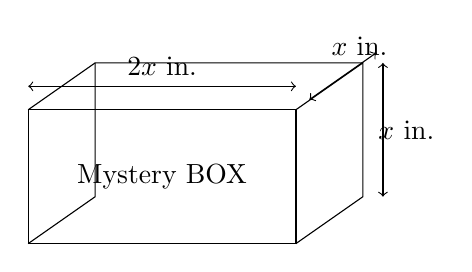
\begin{tikzpicture}[scale=0.85]
\draw (0,0) rectangle (4,2);
\draw (4,0) -- (5,0.7) -- (5,2.7) -- (4,2);
\draw (0,2) -- (1,2.7) -- (5,2.7);
\draw (1,2.7) -- (1,0.7) -- (0,0);
\node at (2,1) {Mystery BOX};
\draw[<->] (0,2.35) -- (4,2.35);
\node at (2,2.65) {\(2x\) in.};
\draw[<->] (4.2,2.15) -- (5.2,2.85);
\node at (4.95,2.95) {\(x\) in.};
\draw[<->] (5.3,0.7) -- (5.3,2.7);
\node at (5.65,1.7) {\(x\) in.};
\end{tikzpicture}

\answer{12 in.}
\end{practice}

\begin{practice}{46}{2}
Make Sense and Persevere Amelia's bank account earns interest annually. The equation shows her starting balance of \$200 and her balance at the end of four years, \$220.82. At what rate, \(r\), did Amelia earn interest?

\[
220.82=200(1+r)^4
\]

\answer{0.025 or 2.5\%}
\end{practice}

\begin{practice}{47}{2}
Model With Mathematics One measure of a patient's body surface area is found using the expression
\[
\sqrt{\frac{H\cdot W}{3,600}}.
\]
Write this with a fractional exponent.

\answer{\(\left(\frac{HW}{3,600}\right)^{\frac12}\)}
\end{practice}

\begin{practice}{48}{1}
Determine if each expression is another way to write \(b^{\frac34}\). Select Yes or No.

\begin{tabular}{lcc}
\toprule
Expression & Yes & No \\
\midrule
a. \(\sqrt[4]{b^3}\) & \(\square\) & \(\square\) \\
b. \((b^3)^{\frac14}\) & \(\square\) & \(\square\) \\
c. \(b^{\frac43}\) & \(\square\) & \(\square\) \\
d. \(\sqrt[3]{b^4}\) & \(\square\) & \(\square\) \\
e. \(\dfrac{b^3}{b^4}\) & \(\square\) & \(\square\) \\
\bottomrule
\end{tabular}

\answer{a. Yes; b. Yes; c. No; d. No; e. No.}
\end{practice}

\begin{practice}{49}{1}
SAT/ACT Which of the following is equivalent to \(\sqrt[6]{4,096x^{18}y^{30}}\), where \(x>0\) and \(y>0\)?

A. \(682.7x^{15}y^{24}\)

B. \(4x^{1.6}y^{1.8}\)

C. \(4,096x^3y^5\)

D. \(4x^3y^5\)

E. \(682.7x^3y^5\)

\answer{D. \(4x^3y^5\)}
\end{practice}

\begin{practice}{50}{3}
Performance Task A milk processing company uses cylindrical-shaped containers. The height of the container is equal to the diameter of the base.

\placeholder{illustration}{Milk processing machine with an orange cylindrical container; label reads "volume 169.65 ft^3."}

Part A How much material is needed to make the lateral surface area of the shipping container?

Part B The cargo hold of a ship is 20 ft high. What is the largest number of these shipping containers that could be stacked on top of each other inside the cargo hold?

\answer{Part A \(36\pi\text{ ft}^2\). Part B 3 containers.}
\end{practice}

\end{document}
```
